\documentclass[journal]{IEEEtran}

\usepackage[T1]{fontenc}
\usepackage{cite}
\usepackage{amsmath,amssymb,amsfonts}
\usepackage{graphicx}
\usepackage{booktabs}
\usepackage{multirow}
\usepackage{array}
\usepackage{microtype}
\usepackage{url}
\usepackage[hidelinks]{hyperref}
\usepackage{tikz}
\usetikzlibrary{arrows.meta,positioning,calc}

\begin{document}

\title{Trust-Aware Joint Adaptive Control and Causal Spatial Reference for Reliable Resource-Constrained IoT Sensing}

\author{Author Name(s) To Be Supplied Before Submission%
\thanks{Manuscript prepared in IEEE Sensors Journal two-column format (\texttt{IEEEtran}). Author names, affiliations, funding acknowledgments, and final ethics/AI disclosures must be supplied by the human author(s) prior to journal submission. Reproducible source code, C11 firmware kernel, hardware-trace archives, and statistical tables are maintained in the TAIS repository.}}

\markboth{IEEE SENSORS JOURNAL, MANUSCRIPT DRAFT (PHASE 5--6 CONSOLIDATION)}%
{Trust-Aware Joint Adaptive Control and Causal Spatial Reference for Reliable IoT Sensing}

\maketitle

\begin{abstract}
Resource-constrained Internet of Things (IoT) monitoring faces two coupled reliability barriers: (i) under lossy low-power wireless links, open-loop adaptive sampling and selective transmission suffer severe Age of Information (AoI) inflation and missed event edges; and (ii) at the single-sensor level, gradual sensor drift is fundamentally confounded with genuine slow environmental changes. We present TAIS-JALC, a lean three-dimensional closed-loop controller integrating frozen C11 sensor-health gating, a bounded 4+1 observation state machine, AoI-sampling hard reservation, and causal link-telemetry redundancy over an unchanged stateless Binary~v1 wire protocol, together with a strictly causal differential spatial $k$-nearest-neighbor ($k$-NN) reference layer. Across 21,000 synthetic boundary runs, TAIS-JALC improves receiver F1 by +10.6 to +11.6 percentage points (pp) over selective fixed-period baselines under 30\% and burst packet loss while capping P95 finite AoI at 42--45\,s. Replayed over 24 real ESP32-S3 + E220-400T22D Sub-GHz hardware loss traces (3,359 RF attempts), TAIS-JALC strictly Pareto-dominates fixed polling (+9.46\,pp F1, $-$46.6\% P95 AoI, $-$54.4\% fault-induced false alarms, and $-$5.1\% RF airtime; all $p_{\text{Holm}} \le 0.0175$). A zero-allocation pure C11 port passes 27/27 bit-exact parity trajectories and compiles for ESP32-S3 (\texttt{-Os}) in 3,328\,B static RAM (including dual-channel health monitoring) and 7,643\,B flash code. Finally, across 12 held-out days of the 54-mote MIT Intel Berkeley dataset (9,000 runs), causal differential spatial $k$-NN cuts drift-induced false environmental alarms by $-$75.0\%, identifies 88.3\% of drifts (96.5\% on normal-coverage days), outperforms an equal-cost \texttt{NullSpatial} negative control by +45.4\,pp on common environmental ramps ($p_{\text{Holm}} = 0.027$), and explicitly quantifies its unidentifiable boundary on single-node slow local events ($-$55.0\,pp).
\end{abstract}

\begin{IEEEkeywords}
Adaptive sampling, Age of Information (AoI), embedded C11, Internet of Things (IoT), LoRa, sensor drift, spatial correlation, wireless sensor networks.
\end{IEEEkeywords}

\section{Introduction}
\IEEEPARstart{L}{ong-lived} wireless sensor networks (WSNs) and edge Internet of Things (IoT) deployments operate at the intersection of three coupled imperfections: low-cost transducers experience stuck readings, range violations, missing samples, and gradual calibration drift~\cite{sharma2010faults,ni2009sensor}; low-power wireless links such as Sub-GHz LoRa suffer bursty packet loss and strict duty-cycle limits~\cite{augustin2016lora,gilbert1960capacity}; and applications require timely, trustworthy state updates quantified by the Age of Information (AoI)~\cite{kaul2012realtime,yates2021age}.

Prior adaptive acquisition and transmission-suppression schemes typically treat these dimensions in isolation~\cite{rao2019adaptive,masoum2012quality,dias2017dual,arnaiz2024energy}. In practice, open-loop coupling fails in two concrete ways. First, when a node suppresses routine uploads to conserve airtime, even moderate wireless packet loss (15\%--30\%) erases event onsets and stretches receiver P95 finite-value AoI past 140--300\,s because lost frames must wait for the next sparse heartbeat. Second, when a single channel undergoes gradual sensor drift, any purely local temporal detector faces a fundamental identifiability deadlock: without external physical context, a slow $+4\,^{\circ}\text{C}$ drift over two hours is observationally indistinguishable from a genuine slow environmental warming ramp.

Equally important in empirical IoT systems research is separating genuine operational gains from simulation artifacts and reporting explicit failure boundaries. Purely synthetic benchmarks conceal non-stationary real-world diurnal heating cycles and real network outages, while unverified Python prototypes do not prove deployability on microcontroller-class hardware.

To address both barriers without bloating protocol or memory overhead, this paper introduces and rigorously evaluates a unified closed-loop observation and causal spatial-reference framework built additively on the open-source TAIS architecture. Our contributions are fourfold:
\begin{enumerate}
\item \textbf{Lean 3D Closed-Loop Control and Zero-Allocation C11 Port:} We design \texttt{TAIS-JALC}, a 4+1 state controller governed by only five primary hyperparameters that couples trust-gated bounded sampling, per-channel AoI-sampling hard reservation, and causal loss-triggered $K{=}2$ critical-edge redundancy while reusing the stateless Binary~v1 frame format unchanged. We implement a zero-heap-allocation pure C11 kernel verified bit-exact against Python across 27 full trajectories and cross-compiled for ESP32-S3 Xtensa LX7 (3.25\,KB combined static RAM, 7.64\,KB controller \texttt{.text}).
\item \textbf{Regime-Boundary Characterization and Real Hardware-Trace Validation:} Across 21,000 synthetic boundary runs (20 sweep + 20 held-out validation seeds) and 2,240 hardware-trace runs replaying 24 audited ESP32-S3 + E220-400T22D Sub-GHz LoRa logs (3,359 physical RF attempts), we establish statistically significant Holm-corrected gains and strict Pareto dominance over fixed polling under real lossy RF traces, alongside explicit failure regimes ($\le 10$\,s pulses, 600\,s ramps, and $7\times$ high-noise events).
\item \textbf{Real 54-Mote External Validity and Causal Differential Spatial Reference:} Auditing 2.31 million raw records from the MIT Intel Berkeley Research Lab 54-mote deployment~\cite{madden2004intel} under a strict chronological split (12 contiguous held-out days, 76.4\% mean coverage, zero future interpolation, retaining a real two-day outage), we evaluate both real-background $\times$ E220 external validity (5,400 runs) and a matched causal differential spatial $k$-NN detector (3,600 runs) that cancels static inter-mote and multi-day seasonal offsets.
\item \textbf{Causal Falsification via Equal-Cost Negative Control and Honest Boundaries:} By pairing \texttt{SpatialKNN} against an equal-cost \texttt{NullSpatial} control (identical code, thresholds, and availability masks, fed calibration-day neighbor readings), we prove that real physical neighbor correlation---not extra computation---drives the +45.4\,pp common-event preservation advantage, while explicitly quantifying both real morning HVAC domain shift and the fundamental single-node slow-local-event unidentifiable boundary (H3).
\end{enumerate}

\section{Related Work}
\paragraph{Adaptive Sampling and Selective Transmission}
Adaptive acquisition modulates sampling intervals based on signal variation, prediction error, or criticality~\cite{rao2019adaptive,masoum2012quality,algabroun2020dsra}. Dual-prediction and deadband upload rules further reduce radio transmissions by omitting routine updates within an error band~\cite{dias2017dual,arnaiz2024energy}. However, when sampling and selective transmission operate open-loop, sparse heartbeats interact destructively with wireless erasures, causing AoI spikes and missed onset edges.

\paragraph{Age of Information and Lossy LPWAN Links}
Age of Information (AoI) captures the freshness of the latest successfully received state at the monitor~\cite{kaul2012realtime,yates2021age}. In Sub-GHz LoRa and ISM-band networks, collisions, fading, and bursty channel memory modeled by Gilbert-Elliott processes~\cite{gilbert1960capacity,augustin2016lora} degrade single-shot transmissions. Most AoI scheduling studies assume trustworthy sensors or abstract packet queues, omitting transducer fault gating and finite-value versus null-frame age semantics.

\paragraph{Sensor Faults and Spatio-Temporal Correlation}
Real-world deployments exhibit frequent stuck-at, out-of-range, spike, missing, and drift faults~\cite{sharma2010faults,ni2009sensor}. Fault-tolerant event detection~\cite{yim2010fault} and cluster-correlated adaptation~\cite{harb2024clara} exploit redundancy across nearby nodes~\cite{vuran2004spatiotemporal,guestrin2004distributed}. Yet many spatial schemes rely on offline regression, non-causal smoothing, or lack equal-cost negative controls to isolate physical correlation from algorithmic complexity. Our work unifies strict causal execution, lightweight C11 closed-loop AoI control, real Sub-GHz hardware loss traces, and equal-cost negative-controlled spatial drift identifiability in a single reproducible study.

\section{System Architecture and Methodology}

Fig.~\ref{fig:arch} illustrates the complete end-to-end architecture combining local closed-loop control (\texttt{TAIS-JALC}) with the gateway/network-level causal differential spatial reference layer. Frozen upstream components---\texttt{SensorTrust} C11 health diagnosis, \texttt{AdaptiveSense} change analysis, and the stateless Binary~v1 wire codec---remain unmodified to guarantee fair comparison against frozen historical baselines.

\begin{figure*}[t]
\centering
\resizebox{0.97\textwidth}{!}{%
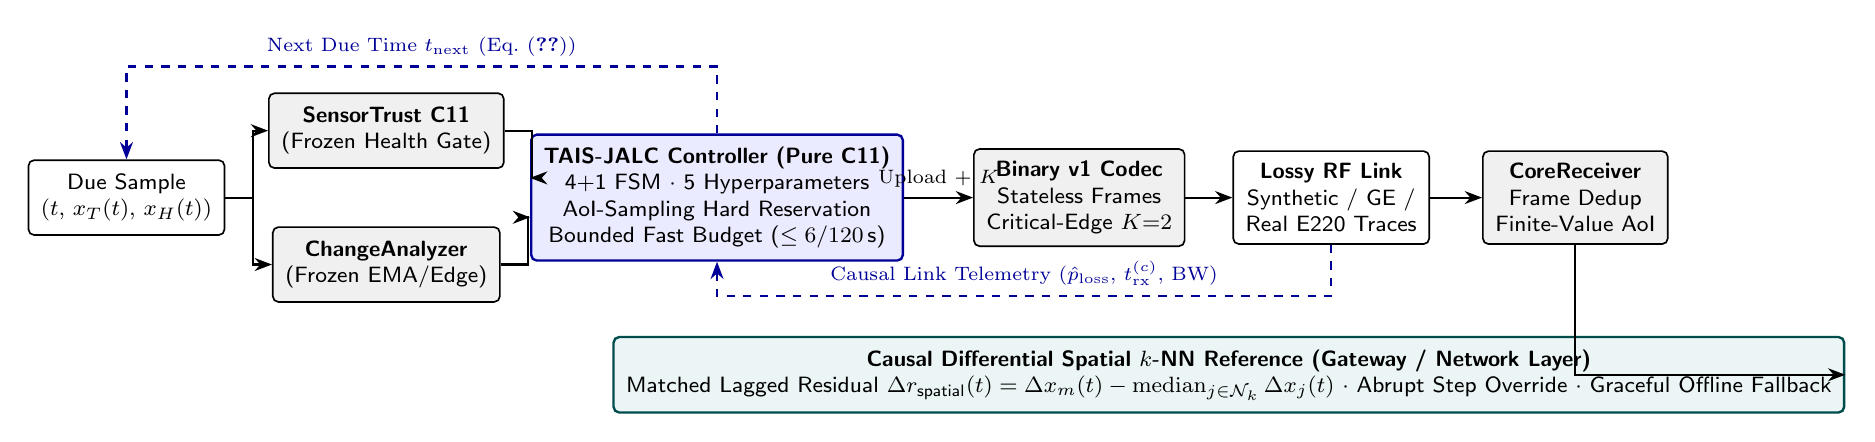
\begin{tikzpicture}[
    font=\sffamily\footnotesize,
    box/.style={draw, rounded corners=2pt, align=center, minimum height=9.5mm, inner sep=4.5pt, fill=white, line width=0.6pt},
    frozen/.style={box, fill=gray!12},
    ctrl/.style={box, fill=blue!8, draw=blue!60!black, line width=0.85pt},
    spatial/.style={box, fill=teal!8, draw=teal!60!black, line width=0.85pt},
    arr/.style={-{Stealth[length=2.2mm]}, line width=0.75pt},
    dasharr/.style={-{Stealth[length=2.2mm]}, dashed, line width=0.75pt, draw=blue!60!black}
]
\node[box] (in) at (0,0) {Due Sample\\$(t,\, x_T(t),\, x_H(t))$};
\node[frozen] (st) at (3.3, 0.85) {\textbf{SensorTrust C11}\\(Frozen Health Gate)};
\node[frozen] (ca) at (3.3,-0.85) {\textbf{ChangeAnalyzer}\\(Frozen EMA/Edge)};
\node[ctrl] (jalc) at (7.5, 0) {\textbf{TAIS-JALC Controller (Pure C11)}\\4+1 FSM $\cdot$ 5 Hyperparameters\\AoI-Sampling Hard Reservation\\Bounded Fast Budget ($\le 6/120$\,s)};
\node[frozen] (v1) at (12.1, 0) {\textbf{Binary v1 Codec}\\Stateless Frames\\Critical-Edge $K{=}2$};
\node[box] (link) at (15.3, 0) {\textbf{Lossy RF Link}\\Synthetic / GE /\\Real E220 Traces};
\node[frozen] (rx) at (18.4, 0) {\textbf{CoreReceiver}\\Frame Dedup\\Finite-Value AoI};
\node[spatial] (sp) at (14.0, -2.25) {\textbf{Causal Differential Spatial $k$-NN Reference (Gateway / Network Layer)}\\Matched Lagged Residual $\Delta r_{\text{spatial}}(t) = \Delta x_m(t) - \operatorname{median}_{j\in\mathcal{N}_k}\Delta x_j(t)$ $\cdot$ Abrupt Step Override $\cdot$ Graceful Offline Fallback};

\draw[arr] (in.east) -- ++(0.35,0) |- (st.west);
\draw[arr] (in.east) -- ++(0.35,0) |- (ca.west);
\draw[arr] (st.east) -- ++(0.35,0) |- ([yshift=2.5mm]jalc.west);
\draw[arr] (ca.east) -- ++(0.35,0) |- ([yshift=-2.5mm]jalc.west);
\draw[arr] (jalc.east) -- node[above, font=\scriptsize]{Upload + $K$} (v1.west);
\draw[arr] (v1.east) -- (link.west);
\draw[arr] (link.east) -- (rx.west);
\draw[arr] (rx.south) |- (sp.east);

\draw[dasharr] (link.south) -- ++(0,-0.65) -| node[pos=0.25, above, font=\scriptsize, text=blue!60!black]{Causal Link Telemetry ($\hat{p}_{\text{loss}}$, $t_{\text{rx}}^{(c)}$, BW)} (jalc.south);
\draw[dasharr] (jalc.north) -- ++(0,0.85) -| node[pos=0.25, above, font=\scriptsize, text=blue!60!black]{Next Due Time $t_{\text{next}}$ (Eq.~\eqref{eq:aoi_reserve})} (in.north);
\end{tikzpicture}%
}
\caption{End-to-end architecture of TAIS-JALC and the causal differential spatial $k$-NN reference layer. Frozen upstream modules (gray) remain untouched; the closed-loop controller (blue) runs in zero-allocation pure C11 on MCU-class nodes, while the causal spatial reference layer (teal) disambiguates slow single-sensor drift from common environmental ramps using physical neighbor streams.}
\label{fig:arch}
\end{figure*}

\subsection{Three-Dimensional Closed-Loop Control (TAIS-JALC)}
At each due timestamp $t$, \texttt{TAIS-JALC} ingests dual-channel readings (temperature and humidity), \texttt{SensorTrust} health states (\texttt{HEALTHY}, \texttt{DEGRADED}, \texttt{FAULT}), \texttt{ChangeAnalyzer} event flags, and causal link feedback. To prevent hyperparameter bloat and overfitting, \texttt{TAIS-JALC} eliminates CUSUM detectors and depends on exactly five frozen primary hyperparameters (Table~\ref{tab:params}).

\begin{table}[t]
\centering
\caption{Frozen Primary Hyperparameters of TAIS-JALC (Phase~5--6)}
\label{tab:params}
\footnotesize
\begin{tabular}{@{}lcl@{}}
\toprule
Parameter & Value & Operational Role \\
\midrule
$I_{\text{fallback}}$ & $20.0\text{\,s}$ & Safe polling floor during noise/cooldown \\
$I_{\text{diag}}$ & $15.0\text{\,s}$ & Diagnostic cadence under \texttt{DEGRADED/FAULT} \\
$T_{\text{AoI}}^{\text{quiet}}$ & $45.0\text{\,s}$ & Hard finite-value AoI cap in quiet regime \\
$T_{\text{AoI}}^{\text{active}}$ & $20.0\text{\,s}$ & Hard finite-value AoI cap in active/probe regime \\
$\theta_{\text{loss}}$ & $0.10$ & Causal loss threshold enabling critical-edge $K{=}2$ \\
\bottomrule
\end{tabular}
\end{table}

\paragraph{Bounded 4+1 Observation State Machine}
The controller transitions deterministically among four nominal states---\texttt{QUIET\_ECO} ($I_{\text{obs}}{=}30$\,s), \texttt{PROBE} ($15$\,s or $5$\,s), \texttt{TRACK} ($5$\,s), and \texttt{SAFE\_FALLBACK} ($I_{\text{fallback}}{=}20$\,s for a 30\,s cooldown)---plus a diagnostic state \texttt{DIAG\_VERIFY} ($I_{\text{diag}}{=}15$\,s) whenever any channel reports \texttt{DEGRADED}, \texttt{FAULT}, or a non-finite reading. Risk scores use robust median/MAD normalization and bounded slope estimates on historical samples. A strict rolling fast-sampling budget permits at most 6 fast samples ($I{<}15$\,s) per 120\,s window; budget exhaustion or 30\,s burst saturation forces transition into \texttt{SAFE\_FALLBACK}, preventing noise-driven sampling runaway.

\paragraph{AoI-Sampling Hard Reservation}
Open-loop upload suppression suffers severe AoI violations whenever a heartbeat deadline falls between sparse samples or when a \texttt{null} (fault-masked) packet resets naive frame age without refreshing finite physical state. \texttt{TAIS-JALC} tracks per-channel last received finite timestamps $t_{\text{rx}}^{(c)}$ strictly ignoring non-finite frames, and injects a hard reservation into the next due sampling instant:
\begin{equation}
t_{\text{next}} = \min\!\Big(t + I_{\text{obs}},\; \max\!\big(t + I_{\min},\; t_{\text{rx}}^{\star} + T_{\text{AoI}}^{\max} - \Delta_{\text{m}}\big)\Big),
\label{eq:aoi_reserve}
\end{equation}
where $t_{\text{rx}}^{\star} = \min_{c \in \mathcal{C}_{\text{fin}}} t_{\text{rx}}^{(c)}$ is the stalest finite channel receipt time, $I_{\min} = 5$\,s, $\Delta_{\text{m}} = 5$\,s, and $T_{\text{AoI}}^{\max} \in \{T_{\text{AoI}}^{\text{quiet}}, T_{\text{AoI}}^{\text{active}}\}$. A sender-side lookahead guard further forces transmission whenever deferring to $t_{\text{next}}$ would breach $T_{\text{AoI}}^{\max}$.

\paragraph{Causal Link Telemetry and Selective Redundancy}
After every transmission attempt, causal link feedback updates an exponentially weighted moving average loss estimate $\hat{p}_{\text{loss}}$ and confirms whether finite values reached the receiver. When $\hat{p}_{\text{loss}} \ge \theta_{\text{loss}} = 0.10$, \texttt{TAIS-JALC} sets redundancy $K{=}2$ exclusively for high-value \texttt{event\_edge} and \texttt{health\_edge} snapshots while keeping ordinary updates at $K{=}1$ (and suppressing non-critical deadband updates during bandwidth congestion). Because the independent \texttt{CoreReceiver} natively deduplicates identical Binary~v1 frames by sequence/timestamp, zero wire-protocol modifications are required. We evaluate three incremental ablation variants: \texttt{JALC-ObsOnly} (4+1 FSM + legacy 120\,s upload), \texttt{JALC-AoI} (adding Eq.~\eqref{eq:aoi_reserve} and per-channel AoI caps), and \texttt{JALC-Full} (complete 3D closed loop with causal link telemetry and critical-edge $K{=}2$).

\subsection{Zero-Allocation Embedded C11 Implementation}
To verify MCU-class feasibility without dynamic memory fragmentation, the complete \texttt{TAIS-JALC} state machine, rolling median/MAD buffers, fast-budget ring buffer, and link telemetry were ported to strict ANSI/ISO C11 (\texttt{src/tais/closed\_loop/c11/tais\_jalc.\{h,c\}}, compiled with \texttt{-std=c11 -Wall -Wextra -Werror}). All buffers are fixed-capacity value structs (\texttt{sizeof(tais\_jalc\_t)} $= 1{,}072$\,B supporting up to 4 channels; zero \texttt{malloc/free}; zero RTOS dependencies). Bit-exact parity against the reference Python implementation was verified over 27 full 1,800\,s trajectories spanning 3 ablation variants $\times$ 3 fault/event scenarios $\times$ 3 link regimes, confirming exact agreement ($<10^{-9}$) on every step's state, upload decision, redundancy $K$, fast-budget counters, and $t_{\text{next}}$.

\subsection{Causal Differential Spatial $k$-NN Reference}
Single-channel detectors cannot distinguish slow sensor drift from genuine slow room-wide warming. Given physical node coordinates $\mathbf{p}_m \in \mathbb{R}^2$, for each target mote $m$ we select its $k{=}4$ nearest physical neighbors $\mathcal{N}_k(m)$ by Euclidean distance (excluding $m$). Critically, static calibration offsets computed days earlier drift under seasonal or solar microclimate changes. Instead, at each discrete slot $t$ (2-min cadence), both target and neighbors compute strictly causal matched lagged deviations over the identical past window $[t{-}L{-}W,\, t{-}L)$ with lag $L{=}20$ (40\,min) and window $W{=}40$ (80\,min):
\begin{align}
\Delta x_m(t) &= x_m(t) - \operatorname{median}\!\big(x_m[t{-}60 : t{-}20]\big), \label{eq:lagdev} \\
\Delta r_{\text{spatial}}(t) &= \Delta x_m(t) - \operatorname{median}_{j \in \mathcal{N}_k^{\text{fresh}}(t)} \Delta x_j(t), \label{eq:spres}
\end{align}
where $\mathcal{N}_k^{\text{fresh}}(t)$ denotes neighbors with finite readings at $t$ and at least 5 finite history points in $[t{-}60:t{-}20)$. Static inter-mote and multi-day baseline offsets cancel identically in Eq.~\eqref{eq:lagdev}--\eqref{eq:spres} with zero future leakage.

To preserve genuine sharp local events (e.g., sudden localized heat or door opening) even during ongoing slow drift, we also compute a strictly causal short-lag jump over $[t{-}8,\, t{-}2)$:
\begin{equation}
a_m(t) = \big|x_m(t) - \operatorname{median}\!\big(x_m[t{-}8 : t{-}2]\big)\big|.
\label{eq:abrupt}
\end{equation}
With consecutive confirmation $c{=}3$ slots (6\,min), thresholds $\tau_{\text{dev}}{=}2.2\,^{\circ}\text{C}$, $\tau_{\text{abrupt}}{=}1.6\,^{\circ}\text{C}$, and $\tau_{\text{sp}}{=}1.4\,^{\circ}\text{C}$ (strictly below $\tau_{\text{dev}}$ to eliminate onset race conditions on slow drifts), the decision rule is:
\begin{enumerate}
\item If $a_m(t) \ge \tau_{\text{abrupt}}$: classify as \textit{environmental event} (preserving local fast events and superimposed drift+fast events).
\item Else if $|\Delta x_m(t)| \ge \tau_{\text{dev}}$ and $|\mathcal{N}_k^{\text{fresh}}(t)| \ge 2$ and $|\Delta r_{\text{spatial}}(t)| \ge \tau_{\text{sp}}$: classify as \textit{single-sensor drift} and suppress false environmental alarm.
\item Else if $|\Delta x_m(t)| \ge \tau_{\text{dev}}$: classify as \textit{environmental event} (confirmed common environmental change, or graceful fallback to \texttt{SingleChannel} during neighbor outages).
\end{enumerate}

\paragraph{Equal-Cost Negative Control (\texttt{NullSpatial})}
To falsify the hypothesis that spatial gains arise from additional computation, smoothing, or availability masking rather than true physical correlation, we construct \texttt{NullSpatial}: it executes the exact same decision code and thresholds with the exact same per-slot neighbor availability mask as \texttt{SpatialKNN}, but substitutes neighbor temperatures from a chronologically disjoint calibration day.

\section{Experimental Setup and Statistical Protocol}

We conduct three strictly separated, seed- and time-isolated campaigns without retuning frozen baselines (\texttt{Fixed-20}, \texttt{A5} = \texttt{Fixed-20+T+U}, \texttt{A7} = native \texttt{AdaptiveSense+T+U}, and \texttt{Risk-T1-U1}):

\begin{enumerate}
\item \textbf{Phase 5 --- Synthetic Boundary Matrix (21,000 runs):} A seed audit across 388 historical manifests confirmed zero overlap with sweep seeds \texttt{1020--1039} and held-out validation seeds \texttt{1100--1119} (20 seeds $\times$ 75 conditions $\times$ 7 methods each): Axis~A ($5\times 5$ event duration $10$--$600$\,s $\times$ amplitude $0.5\times$--$2.5\times$), Axis~B ($5\times 3$ packet loss $0\%$--$30\%$ + Gilbert-Elliott burst fading $\times$ bandwidth caps unlimited / 1200 / 600\,B/min), and Slice~C ($7\times$ noise and same/cross-channel faults at 0\% and 15\% loss).
\item \textbf{Phase 5.5 --- Real ESP32-S3 + E220 Hardware Traces (2,240 runs):} We extracted 24 audited hardware runs (3,359 physical RF attempts; SHA-256 verified) from dual ESP32-S3 + E220-400T22D Sub-GHz LoRa nodes across four measured regimes (\texttt{e220\_random\_20}: 21.17\% loss; \texttt{e220\_random\_30}: 31.72\%; \texttt{e220\_burst\_20}: 19.15\%, max 9-frame burst; \texttt{e220\_burst\_30}: 28.02\%, max 12-frame burst; measured TX airtime 30.4\,ms/frame, ACK RTT 743.1\,ms) and replayed them on isolated held-out seeds \texttt{1200--1219}.
\item \textbf{Phase 6 --- MIT Intel Berkeley 54-Mote Dataset (9,000 runs):} Stream-auditing all 2,313,682 raw lines of \texttt{data.txt.gz} removed 93,879 malformed rows, 9,719 unknown motes, 384,505 out-of-range temperatures, and 289,176 invalid humidities, yielding 1,816,504 valid T+RH records across 54 located motes (zero future interpolation; missing slots remain \texttt{None}). Under a pre-declared chronological split---calibration prefix (\texttt{2004-02-28} to \texttt{03-01}, 83.8\%--89.3\% coverage), 1-day isolation gap (\texttt{03-02}), and 12 contiguous held-out days (\texttt{2004-03-03} to \texttt{03-14})---mean 54-mote 2-min coverage is \textbf{76.4\%}, passing our $\ge 50\%$ coverage gate while intentionally retaining the real March~10--11 outage (31.1\% and 47.8\% coverage). Target motes (top-10 for Exp~A, top-20 for Exp~B; mean $k{=}4$ neighbor distance $5.09 \pm 0.74$\,m) were selected strictly from calibration counts.
\begin{itemize}
\item \textit{Exp~A (5,400 runs):} 12 held-out dates $\times$ 10 motes $\times$ 3 controlled scenarios (\texttt{real\_clean\_events}, \texttt{real\_range\_cross}, \texttt{real\_drift\_cross}) $\times$ 3 links (\texttt{loss\_0}, \texttt{e220\_burst\_20}, \texttt{e220\_random\_30}) $\times$ 5 methods, mapping 3 real hours (\texttt{08:00--11:00}, 30\,s slots) 1:6 to TAIS 5\,s ticks with all reported AoI converted back to real wall-clock seconds.
\item \textit{Exp~B (3,600 runs):} 12 held-out dates $\times$ 20 motes $\times$ 5 scenarios (\texttt{single\_drift}, \texttt{common\_env\_event}, \texttt{local\_fast\_event}, \texttt{drift\_plus\_local\_fast}, and \texttt{local\_slow\_event}) $\times$ 3 causal detectors (\texttt{SingleChannel}, \texttt{SpatialKNN}, \texttt{NullSpatial}) over full \texttt{06:00--20:00} real days (420 causal 2-min slots; daytime interventions at \texttt{11:00--15:00} with $+4.0\,^{\circ}\text{C}$ 2-h ramps and $+3.5\,^{\circ}\text{C}$ 40-min fast steps).
\end{itemize}
\end{enumerate}

\paragraph{Statistical Inference}
All uncertainty intervals use cluster-paired bootstrap (5,000 resamples; seed clusters in Phases~5/5.5, date clusters in Phase~6) paired with exact two-sided cluster sign-flip tests (20,000 permutations) and Holm-Bonferroni correction~\cite{holm1979simple} across every prespecified test family ($\alpha = 0.05$).

\section{Experimental Results}

\subsection{Phase 5: Synthetic Effective and Failure Boundaries}

Fig.~\ref{fig:p5_axis_a} maps receiver F1 across the $5\times 5$ event duration $\times$ amplitude grid. On short-to-medium events ($D \in [20, 45]$\,s, amplitude $\ge 0.75\times$), \texttt{JALC-Full} lifts held-out F1 by \textbf{+8.6 to +24.5\,pp} over \texttt{A5} (e.g., at $D{=}20$\,s, $1.5\times$: 33.9\% vs.\ 9.4\%; at $D{=}45$\,s, $2.5\times$: 71.1\% vs.\ 53.0\%). Fig.~\ref{fig:p5_axis_a} also exposes two sharp failure edges: ultra-short pulses ($D{\le}10$\,s) fail across all policies due to the frozen 10\,s debounce in \texttt{ChangeAnalyzer}, while smooth 600\,s ramps ($\le 1.5\times$) are absorbed by the frozen 60\,s EMA baseline (0\% recall across all policies).

\begin{figure*}[t]
\centering
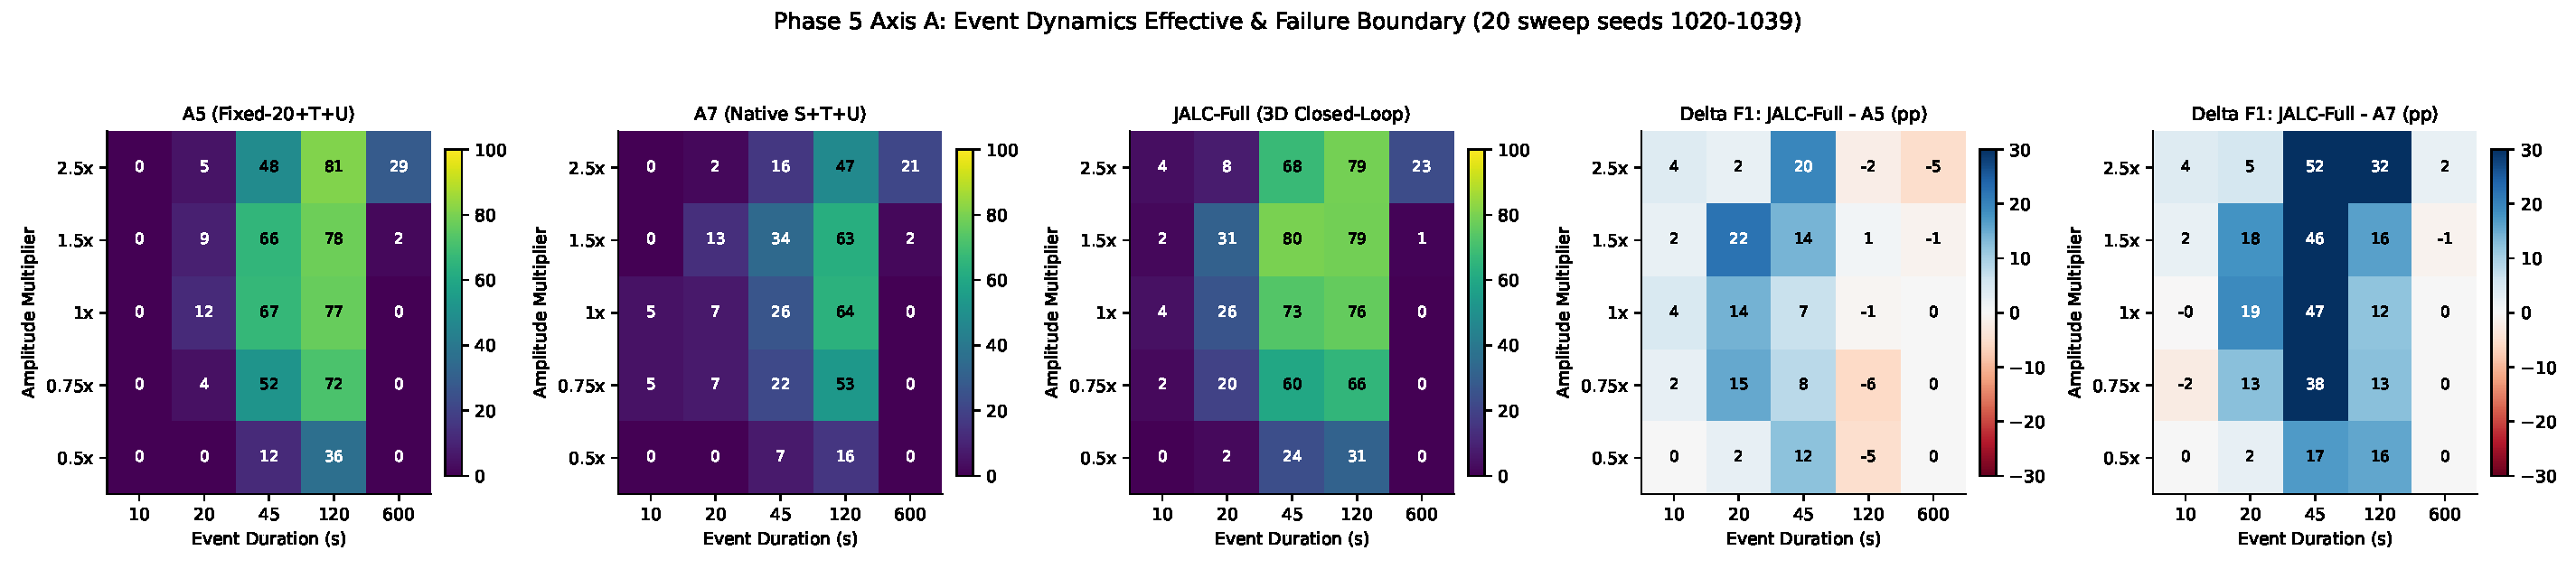
\includegraphics[width=0.96\textwidth]{../../results/phase5/analysis/figures/fig01_axis_a_dynamics_phase_map.pdf}
\caption{Phase~5 Axis~A event-dynamics phase map ($5\times 5$ duration $\times$ amplitude grid, 20 sweep seeds \texttt{1020--1039}). \texttt{JALC-Full} delivers substantial gains on 20--45\,s events while transparently exposing the $\le 10$\,s short-pulse and 600\,s slow-ramp boundaries.}
\label{fig:p5_axis_a}
\end{figure*}

Fig.~\ref{fig:p5_axis_b} and Table~\ref{tab:p5_summary} report held-out validation results (\texttt{1100--1119}). Under 0\% loss, \texttt{JALC-Full} matches \texttt{A5} in F1 ($+0.61$\,pp, $p_{\text{Holm}}{=}1.0$) while cutting P95 finite AoI by 61.6\% (105.4\,s $\to$ 40.5\,s, 0.00\% violation). Once packet loss reaches $\ge 15\%$ or Gilbert-Elliott burst fading, open-loop sparse baselines suffer AoI collapse (P95 rising to 140--190\,s) and missed event edges, whereas \texttt{JALC-Full} achieves Holm-significant F1 gains of \textbf{+11.55\,pp} over \texttt{A5} and \textbf{+11.28\,pp} over \texttt{Fixed-20} at 30\% loss ($p_{\text{Holm}} \le 0.046$) and \textbf{+10.61\,pp} under burst fading ($p_{\text{Holm}} = 0.020$), holding P95 finite AoI at 41.9\,s across Axis~B. In Slice~C, \texttt{JALC-Full} maintains non-degraded operational fault-induced false alarms (FI = 61 vs.\ 72 for \texttt{A5} and 240 for \texttt{Fixed-20}, $p_{\text{Holm}} = 0.020$) and reduces $7\times$ noise-only sampling by $-$69.9\% relative to \texttt{A7}; honestly, under $7\times$ noisy events, MAD scaling plus the 6/120\,s fast cap lowers \texttt{JALC-Full} recall (48.3\% vs.\ 58.3\% for \texttt{A5}).

\begin{figure*}[t]
\centering
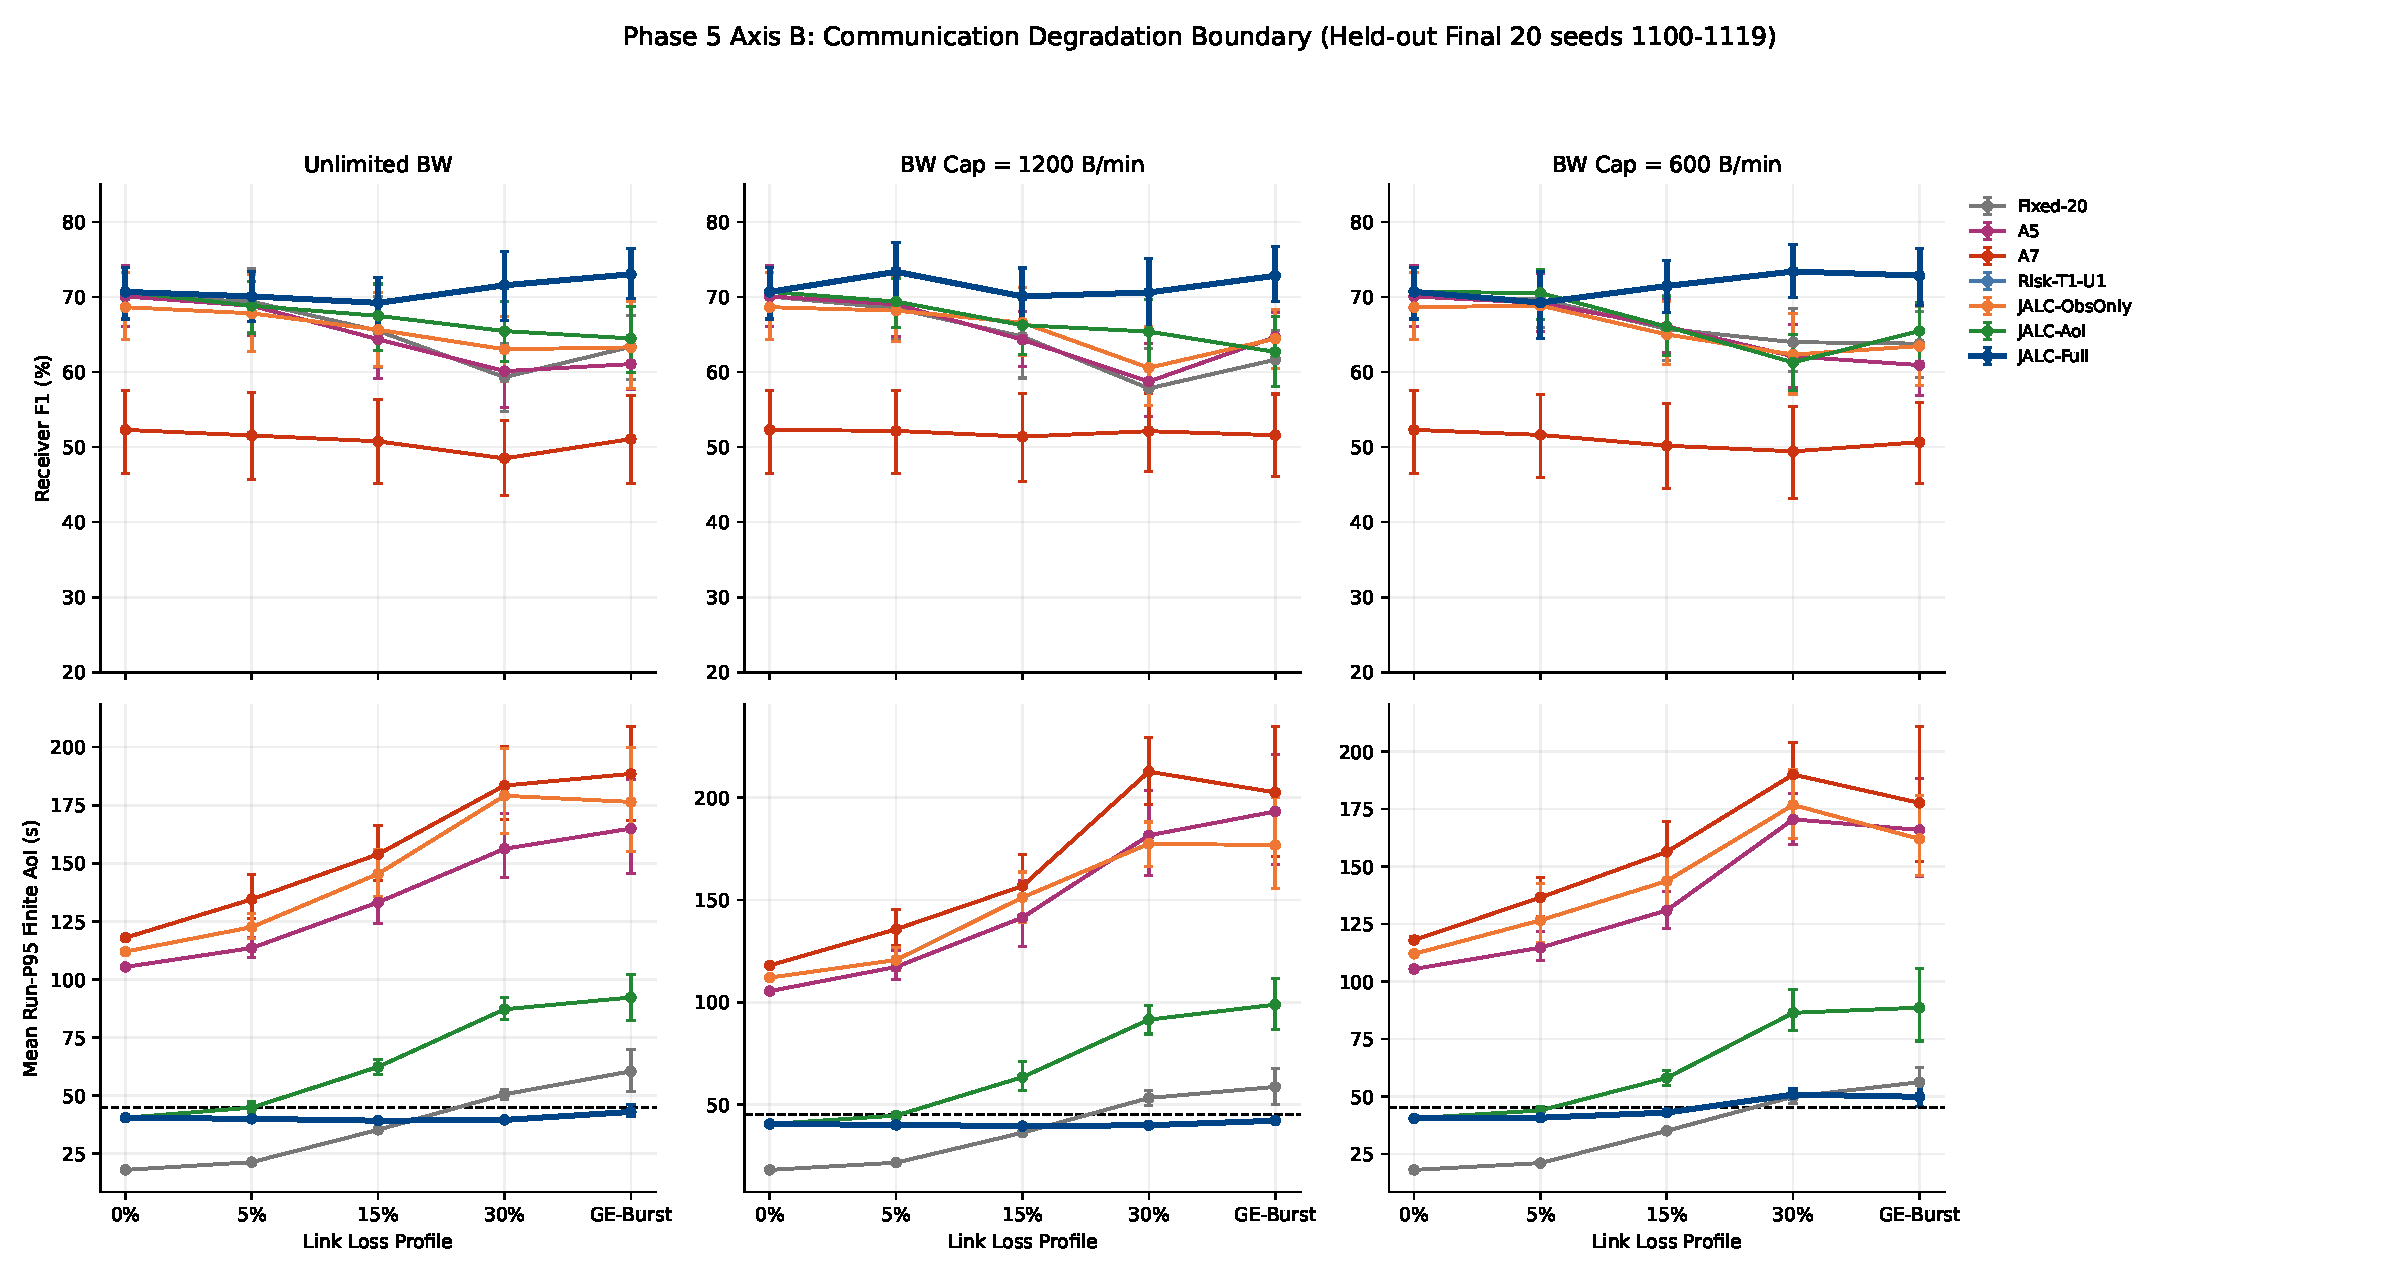
\includegraphics[width=0.95\textwidth]{../../results/phase5/analysis/figures/fig02_axis_b_link_degradation_boundary.pdf}
\caption{Phase~5 Axis~B communication degradation boundary (20 held-out seeds \texttt{1100--1119}) across 0\%--30\% random loss, Gilbert-Elliott burst fading, and bandwidth caps (unlimited, 1200, and 600\,B/min). Error bars show 95\% seed-cluster bootstrap CIs.}
\label{fig:p5_axis_b}
\end{figure*}

\begin{table}[t]
\centering
\caption{Phase~5 Held-Out Validation Summary (Seeds \texttt{1100--1119})}
\label{tab:p5_summary}
\scriptsize
\setlength{\tabcolsep}{3.2pt}
\begin{tabular}{@{}llcccccc@{}}
\toprule
Group & Method & Rx F1 & Recall & P95 AoI & Viol. & Bytes & Rx FI \\
 & & (\%) & (\%) & (s) & (\%) & (kB) & \\
\midrule
\multirow{4}{*}{\shortstack[l]{Axis A\\Dyn.}}
 & Fixed-20 & 36.00 & 27.45 & 18.05 & 0.00 & 1616.5 & 0 \\
 & A5 & 32.06 & 24.55 & 107.09 & 43.22 & 534.8 & 0 \\
 & A7 & 23.80 & 16.55 & 113.40 & 50.46 & 525.8 & 0 \\
 & \textbf{JALC-Full} & \textbf{37.23} & \textbf{29.45} & \textbf{40.92} & \textbf{0.00} & 995.5 & 0 \\
\midrule
\multirow{5}{*}{\shortstack[l]{Axis B\\Links}}
 & Fixed-20 & 66.29 & 53.50 & 36.91 & 3.30 & 1939.8 & 0 \\
 & A5 & 65.94 & 52.93 & 139.97 & 42.87 & 805.3 & 0 \\
 & A7 & 52.49 & 43.74 & 158.83 & 47.53 & 1162.3 & 0 \\
 & JALC-AoI & 67.49 & 57.67 & 65.56 & 9.03 & 1465.8 & 0 \\
 & \textbf{JALC-Full} & \textbf{71.70} & \textbf{63.24} & \textbf{41.94} & \textbf{1.77} & 1763.7 & 0 \\
\midrule
\multirow{4}{*}{\shortstack[l]{Slice C\\Faults}}
 & Fixed-20 & 47.14 & 46.82 & 33.17 & 1.42 & 1276.1 & 240 \\
 & A5 & 49.49 & 45.53 & 112.22 & 36.90 & 586.4 & 72 \\
 & JALC-AoI & 52.54 & 47.80 & 54.87 & 4.83 & 937.9 & 55 \\
 & \textbf{JALC-Full} & \textbf{54.49} & \textbf{50.83} & \textbf{44.53} & \textbf{0.93} & 1032.0 & \textbf{61} \\
\bottomrule
\end{tabular}
\end{table}

\subsection{Phase 5.5: Real E220 Hardware Traces and C11 Footprint}

Fig.~\ref{fig:p55_e220} and Table~\ref{tab:p55_hw} summarize the 2,240-run replay over real ESP32-S3 + E220-400T22D Sub-GHz hardware traces (\texttt{1200--1219}). Across all four measured E220 regimes, \texttt{JALC-Full} achieves \textbf{strict multi-objective Pareto dominance} over \texttt{Fixed-20}: \textbf{+9.46\,pp} receiver F1 ($p_{\text{Holm}}{=}0.0063$), \textbf{$-$40.47\,s} ($-$46.6\%) P95 finite AoI ($p_{\text{Holm}}{=}0.0063$), \textbf{$-$54.4\%} operational FI (78 vs.\ 171, $p_{\text{Holm}}{=}0.0063$), and \textbf{$-$5.1\%} lower measured physical E220 RF airtime (41.61\,s vs.\ 43.84\,s/seed). Compared with open-loop \texttt{A5}, \texttt{JALC-Full} lifts F1 by \textbf{+7.74\,pp} ($p_{\text{Holm}}{=}0.0175$) and slashes P95 AoI by \textbf{$-$179.53\,s} (225.92\,s $\to$ 46.39\,s, $p_{\text{Holm}}{=}0.0063$) with non-degraded FI ($p_{\text{Holm}}{=}1.0$). Under the harshest \texttt{e220\_burst\_30} regime (up to 12 consecutive lost frames), \texttt{A5} P95 AoI collapses to 321--324\,s whereas \texttt{JALC-Full} holds 60.52\,s. Transparently, this freshness guarantee requires 41.61\,s/seed of RF airtime versus 16.45\,s/seed for freshness-blind \texttt{A5}.

\begin{figure*}[t]
\centering
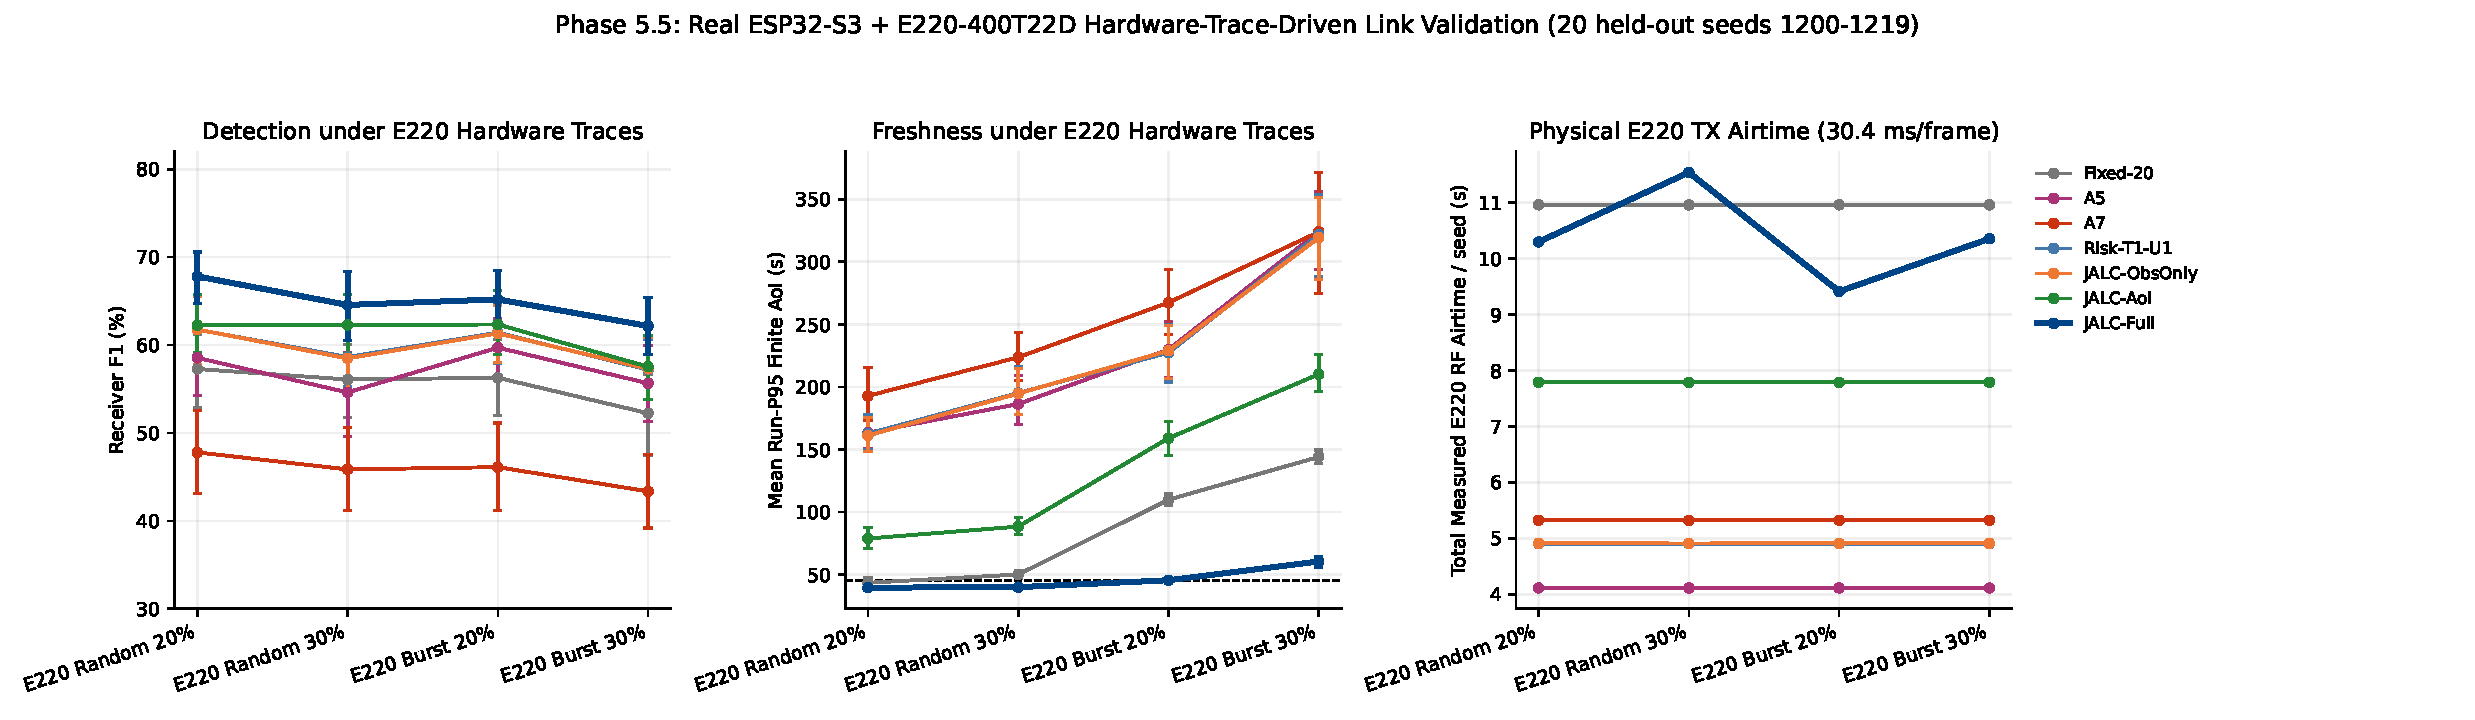
\includegraphics[width=0.95\textwidth]{../../results/phase5_hw_trace/fig05_e220_hardware_trace_validation.pdf}
\caption{Phase~5.5 hardware-trace validation (20 held-out seeds \texttt{1200--1219}) replaying 24 audited ESP32-S3 + E220-400T22D Sub-GHz logs: receiver F1 (left), P95 finite AoI (center), and measured physical E220 RF airtime at 30.4\,ms/frame (right).}
\label{fig:p55_e220}
\end{figure*}

\begin{table}[t]
\centering
\caption{Phase~5.5 Real E220 Hardware-Trace Summary (All 4 Regimes, Seeds \texttt{1200--1219})}
\label{tab:p55_hw}
\scriptsize
\setlength{\tabcolsep}{3.0pt}
\begin{tabular}{@{}lccccccc@{}}
\toprule
Method & Rx F1 & Recall & P95 AoI & Viol. & Bytes & Airtime & Rx FI \\
 & (\%) & (\%) & (s) & (\%) & (kB) & (s/seed) & \\
\midrule
Fixed-20 & 56.09 & 45.78 & 86.86 & 12.05 & 1027.6 & 43.84 & 171 \\
A5 & 57.62 & 45.31 & 225.92 & 51.98 & 385.9 & 16.45 & 75 \\
A7 & 46.96 & 36.77 & 251.96 & 55.37 & 500.6 & 21.29 & 58 \\
Risk-T1-U1 & 60.24 & 49.17 & 226.72 & 52.51 & 460.3 & 19.62 & 67 \\
JALC-AoI & 61.61 & 51.15 & 134.11 & 19.41 & 730.4 & 31.15 & 70 \\
\textbf{JALC-Full} & \textbf{65.33} & \textbf{57.66} & \textbf{46.39} & \textbf{3.25} & \textbf{975.1} & \textbf{41.61} & \textbf{78} \\
\bottomrule
\end{tabular}
\end{table}

Table~\ref{tab:c11} summarizes the pure C11 resource footprint. Cross-compiled with \texttt{xtensa-esp-elf-gcc 14.2.0 -Os}, the combined controller and dual-channel \texttt{SensorTrust} engine occupy only \textbf{3,328\,B (3.25\,KB)} of static RAM ($0.65\%$ of ESP32-S3's 512\,KB SRAM), \textbf{9,662\,B (9.44\,KB)} of flash \texttt{.text}, and \textbf{0\,B} of heap or static \texttt{.data/.bss}, executing at 1.44\,$\mu$s/step on an Apple arm64 host (694,228 updates/s).

\begin{table}[t]
\centering
\caption{Zero-Allocation Pure C11 Footprint and ESP32-S3 Metrics}
\label{tab:c11}
\scriptsize
\setlength{\tabcolsep}{4pt}
\begin{tabular}{@{}lc@{}}
\toprule
Metric (\texttt{-std=c11 -Wall -Wextra -Werror}) & Measured Value \\
\midrule
Controller RAM (\texttt{sizeof(tais\_jalc\_t)}, $\le 4$ ch.) & \textbf{1,072\,B} (0\,B heap) \\
Total RAM (\texttt{tais\_jalc\_t} + $2{\times}$\texttt{sensor\_trust\_t}) & \textbf{3,328\,B} (3.25\,KB) \\
ESP32-S3 \texttt{-Os} flash (\texttt{tais\_jalc} / \texttt{sensor\_trust}) & \textbf{7,643\,B} / \textbf{2,019\,B} \\
ESP32-S3 static \texttt{.data} / \texttt{.bss} & \textbf{0\,B} / \textbf{0\,B} \\
Host joint latency (100k iters, arm64 \texttt{-O2}) & \textbf{1.44\,$\mu$s} (P99: 3.0\,$\mu$s) \\
Python--C11 bit-exact parity ($<10^{-9}$) & \textbf{27 / 27} trajectories \\
\bottomrule
\end{tabular}
\end{table}

\subsection{Phase 6: 54-Mote External Validity and Spatial Identifiability}

\paragraph{Exp~A --- Real Sensing Background $\times$ Real E220 Traces}
Fig.~\ref{fig:p6_expa} shows the pre-evaluation coverage audit (passing the 50\% gate at 76.4\% over 12 contiguous held-out days) and Exp~A external validity (5,400 runs). Under \texttt{e220\_random\_30}, \texttt{JALC-Full} slashes real wall-clock P95 finite AoI from \textbf{2,225.3\,s (37.1\,min)} for \texttt{A5} to \textbf{1,313.4\,s (21.9\,min)} ($-$911.8\,s, $p_{\text{Holm}}{=}0.0258$), cuts AoI violation by \textbf{$-$44.2\,pp} ($p_{\text{Holm}}{=}0.0258$), beats \texttt{Fixed-20} on P95 AoI ($-$94.6\,s, $p_{\text{Holm}}{=}0.0273$) and violation ($-$5.7\,pp, $p_{\text{Holm}}{=}0.0258$) with lower byte volume (990 vs.\ 1,072\,kB) and lower FI (304 vs.\ 364), and raises recall by \textbf{+15.6\,pp} (79.38\% vs.\ 63.75\%).

Crucially, Exp~A also reveals an honest real-world domain shift: Intel Berkeley rooms experience rapid morning HVAC/solar warming ($+5.3$ to $+9.7\,^{\circ}\text{C}$ between \texttt{06:00} and \texttt{12:00}). Because the frozen synthetic \texttt{noise\_floor = 0.15\,$^{\circ}$C} was intentionally not retuned, natural morning warming triggers unlabelled background alarms in high-recall policies, leaving overall F1 statistically indistinguishable from \texttt{A5} (55.30\% vs.\ 55.84\%, $p_{\text{Holm}}{=}1.0$). This finding motivates spatial reference for non-stationary real backgrounds.

\begin{figure*}[t]
\centering
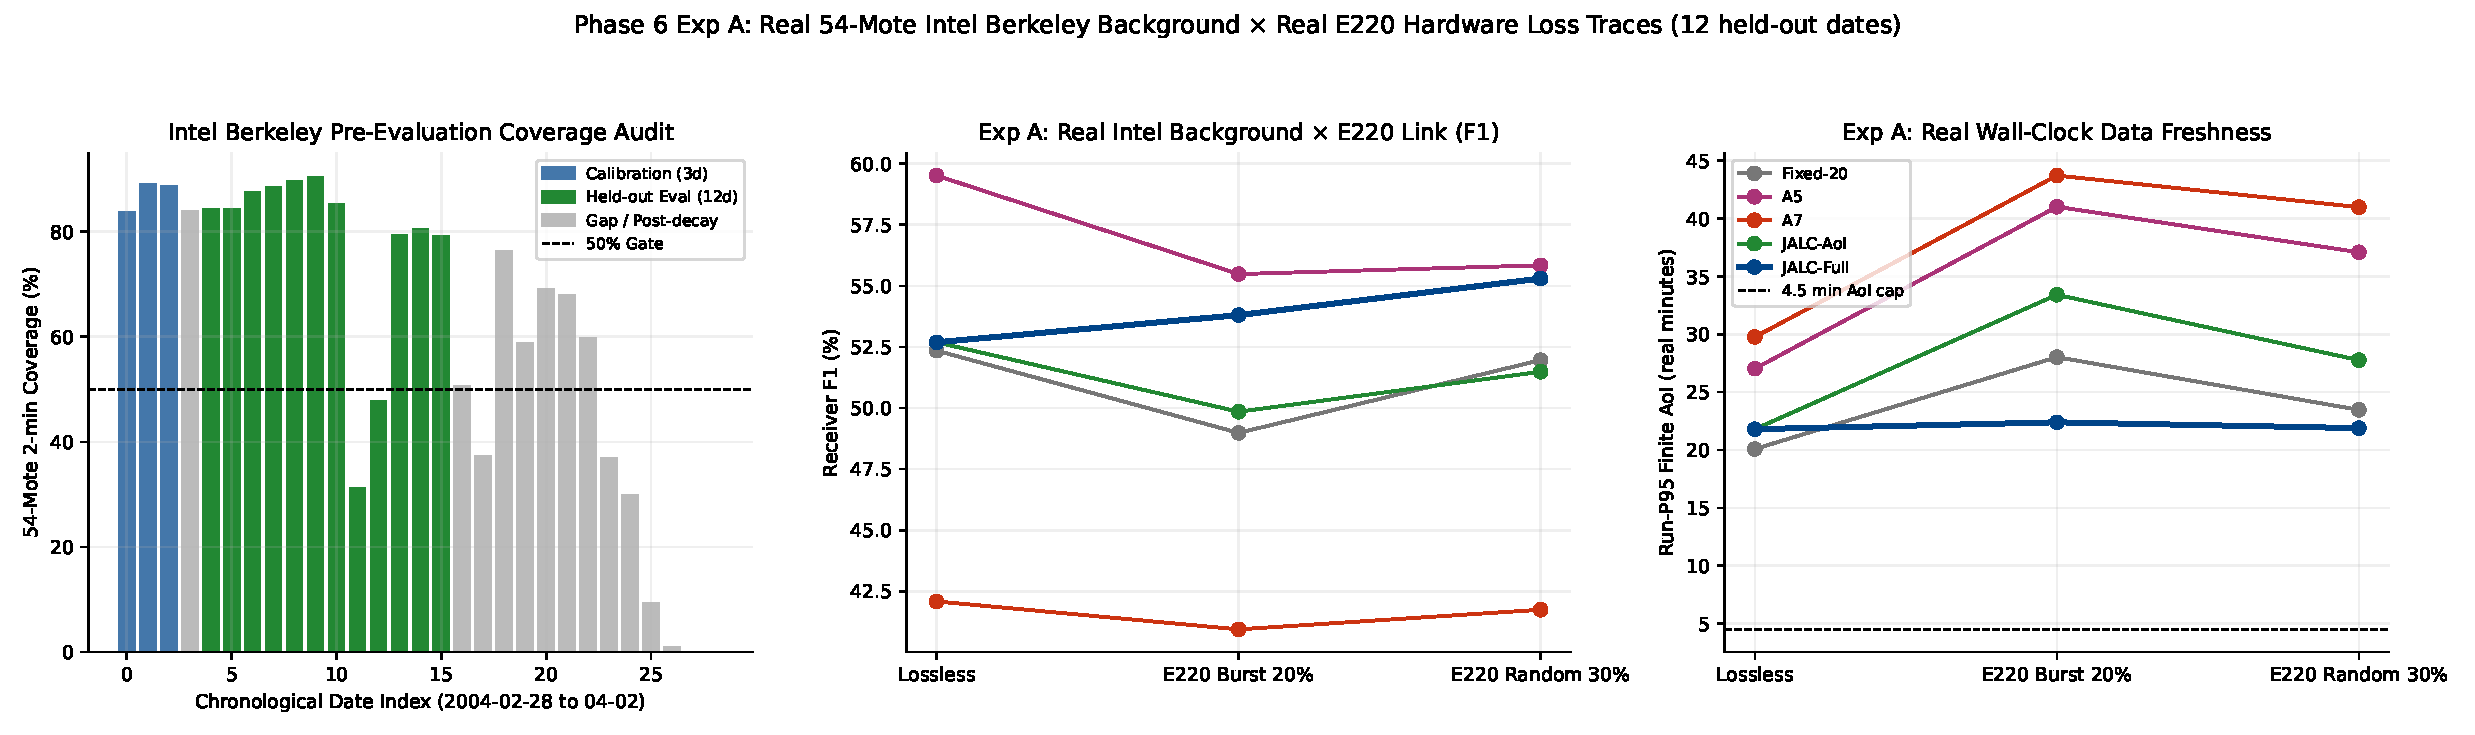
\includegraphics[width=0.96\textwidth]{../../results/phase6_intel_berkeley/figures/fig01_intel_berkeley_coverage_and_external_validity.pdf}
\caption{Phase~6 Exp~A: MIT Intel Berkeley 54-mote pre-evaluation coverage audit (left; blue = 3-day calibration, green = 12-day held-out block including real March~10--11 outage) and external validity across lossless, \texttt{e220\_burst\_20}, and \texttt{e220\_random\_30} hardware traces (center/right).}
\label{fig:p6_expa}
\end{figure*}

\paragraph{Exp~B --- Causal Differential Spatial $k$-NN vs.\ Equal-Cost \texttt{NullSpatial}}
Fig.~\ref{fig:p6_expb} and Table~\ref{tab:p6_expb} report all 3,600 held-out runs across 12 dates $\times$ 20 motes. Four findings stand out with strict date-cluster Holm significance:
\begin{enumerate}
\item \textbf{Single-Mote Drift Suppression (H1):} \texttt{SpatialKNN} cuts drift-induced false environmental alarms by \textbf{$-$75.0\%} relative to \texttt{SingleChannel} (1.583 $\to$ 0.396/run, $p_{\text{Holm}}{=}0.0270$) while correctly identifying \textbf{88.33\%} of single-mote drifts (\textbf{96.5\%} on the 10 normal-coverage days vs.\ 0.0\% for \texttt{SingleChannel}, $p_{\text{Holm}}{=}0.0270$).
\item \textbf{Equal-Cost Negative Control Falsification:} On \texttt{common\_env\_event}, \texttt{SpatialKNN} preserves \textbf{85.83\%} event recall with \textbf{0.00\,pp} degradation versus \texttt{SingleChannel} (95\% CI $[0.0, 0.0]$), whereas equal-cost \texttt{NullSpatial} (using identical code and 344.85 vs.\ 344.87 reference slots/day) collapses to \textbf{40.42\%} (\textbf{+45.42\,pp} advantage for \texttt{SpatialKNN}, $p_{\text{Holm}}{=}0.0270$). On completely unperturbed clean days, \texttt{SpatialKNN} also emits \textbf{$-$63.8\%} fewer spurious drift flags than \texttt{NullSpatial} (0.783 vs.\ 2.167/run, $p_{\text{Holm}}{=}0.0258$).
\item \textbf{Superimposed Drift + Fast Local Events (H2):} When a $+3.5\,^{\circ}\text{C}$ fast local event arrives during an active slow drift, \texttt{SingleChannel} is already saturated by false drift alarms (23.33\% recall), whereas \texttt{SpatialKNN} suppresses the drift ($-$65.9\% false alarms, $p_{\text{Holm}}{=}0.0270$) and recovers \textbf{88.33\%} event recall (\textbf{+65.00\,pp}, $p_{\text{Holm}}{=}0.0270$; \textbf{96.5\%} on normal days).
\item \textbf{Real Outage Graceful Fallback and Honest H3 Boundary:} During the real March~10--11 outage, available spatial reference slots fall by 56\% (380.7 $\to$ 165.9/day), yet \texttt{SpatialKNN} gracefully matches \texttt{SingleChannel}'s 47.5\% event recall floor without crashing or suppressing valid events. Finally, on \texttt{local\_slow\_event} (a slow $+4\,^{\circ}\text{C}$ ramp confined strictly to a single mote), \texttt{SpatialKNN} recall drops by \textbf{$-$55.00\,pp} (85.83\% $\to$ 30.83\%, $p_{\text{Holm}}{=}0.0270$), empirically confirming the fundamental physical unidentifiability of single-node slow local events under single-modality spatial comparison.
\end{enumerate}

\begin{figure*}[t]
\centering
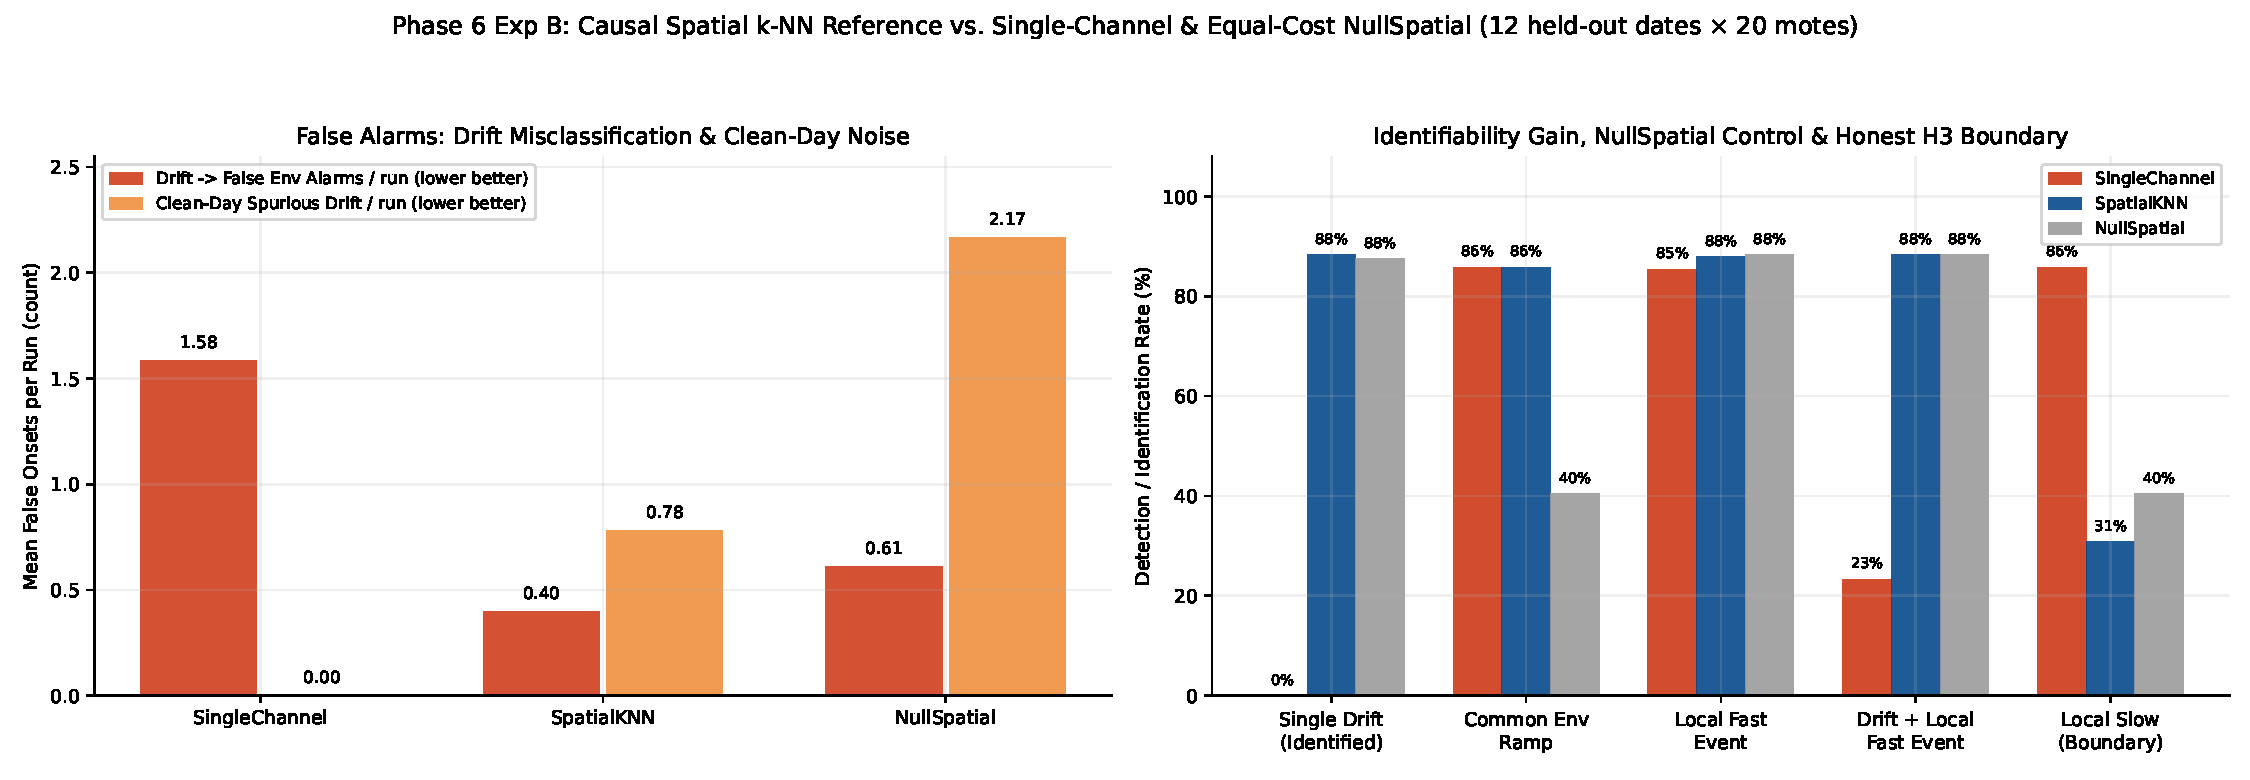
\includegraphics[width=0.96\textwidth]{../../results/phase6_intel_berkeley/figures/fig02_spatial_identifiability_drift_vs_events.pdf}
\caption{Phase~6 Exp~B (12 held-out dates $\times$ 20 motes): drift misclassification and clean-day spurious drift rates (left), alongside drift identification, common-event preservation versus equal-cost \texttt{NullSpatial}, superimposed drift+fast recovery, and the honest \texttt{local\_slow\_event} H3 boundary (right).}
\label{fig:p6_expb}
\end{figure*}

\begin{table*}[t]
\centering
\caption{Phase~6 Exp~B: Causal Spatial $k$-NN vs.\ SingleChannel and Equal-Cost NullSpatial (12 Held-Out Dates $\times$ 20 Motes)}
\label{tab:p6_expb}
\scriptsize
\setlength{\tabcolsep}{4.5pt}
\begin{tabular}{@{}llccccc@{}}
\toprule
Scenario (240 runs each) & Metric & SingleChannel & SpatialKNN & NullSpatial & SpatialKNN Paired Effect (95\% Date-Cluster CI) & $p_{\text{Holm}}$ \\
\midrule
\texttt{single\_drift} (H1) & False env / run $\downarrow$ & 1.583 & \textbf{0.396} & 0.613 & vs.\ SC: \textbf{$-$1.188} ($[-1.525,\,-0.846]$) & \textbf{0.0270} \\
\texttt{single\_drift} (H1) & Drift ID (\%) $\uparrow$ & 0.0 & \textbf{88.3} (96.5$^\dagger$) & 87.5 & vs.\ SC: \textbf{+88.3\,pp} ($[+71.3,\,+97.9]$) & \textbf{0.0270} \\
Clean unperturbed days & Spurious drift / run $\downarrow$ & 0.000 & \textbf{0.783} & 2.167 & vs.\ Null: \textbf{$-$1.383} ($[-1.804,\,-0.954]$) & \textbf{0.0258} \\
\texttt{common\_env\_event} (H1) & Event recall (\%) $\uparrow$ & 85.8 & \textbf{85.8} (93.5$^\dagger$) & 40.4 & vs.\ Null: \textbf{+45.4\,pp} ($[+32.5,\,+59.2]$); vs.\ SC: 0.0 & \textbf{0.0270} \\
\texttt{local\_fast\_event} (H2) & Event recall (\%) $\uparrow$ & 85.4 & \textbf{87.9} (96.0$^\dagger$) & 88.3 & vs.\ SC: +2.5\,pp ($[+0.8,\,+4.2]$) & 1.0000 \\
\texttt{drift\_plus\_local\_fast} (H2) & Event recall (\%) $\uparrow$ & 23.3 & \textbf{88.3} (96.5$^\dagger$) & 88.3 & vs.\ SC: \textbf{+65.0\,pp} ($[+46.3,\,+81.7]$) & \textbf{0.0270} \\
\texttt{drift\_plus\_local\_fast} (H2) & Drift false env / run $\downarrow$ & 0.575 & \textbf{0.196} & 0.271 & vs.\ SC: \textbf{$-$0.379} ($[-0.533,\,-0.238]$) & \textbf{0.0270} \\
\texttt{local\_slow\_event} (H3) & Event recall (\%) & 85.8 & \textbf{30.8} (35.5$^\dagger$) & 40.4 & vs.\ SC: \textbf{$-$55.0\,pp} ($[-68.3,\,-40.8]$) [H3 Bound] & \textbf{0.0270} \\
\bottomrule
\multicolumn{7}{@{}l}{\scriptsize $^\dagger$Stratified performance on the 10 normal-coverage held-out days (excluding the real March~10--11 outage days, where \texttt{SpatialKNN} gracefully matches SC at 47.5\% recall).}
\end{tabular}
\end{table*}

\section{Discussion, Limitations, and Operational Boundaries}

Table~\ref{tab:regimes} synthesizes our findings into an actionable deployment boundary guide. Rather than claiming universal optimality, our evidence defines clear operating regimes:

\begin{table}[t]
\centering
\caption{Operational Regime Matrix and Documented Failure Boundaries}
\label{tab:regimes}
\scriptsize
\setlength{\tabcolsep}{3.5pt}
\begin{tabular}{@{} >{\raggedright\arraybackslash}p{2.15cm} >{\raggedright\arraybackslash}p{1.65cm} >{\raggedright\arraybackslash}p{3.75cm} @{}}
\toprule
Operating Regime & Recommended & Empirical Evidence \\
\midrule
Lossy/bursty links ($\ge 15\%$) + AoI SLA & \texttt{JALC-Full} & +7.7 to +11.6\,pp F1, 42--46\,s P95 AoI, strict Pareto win over \texttt{Fixed-20} on E220 traces \\
Short--medium bursts ($20$--$45$\,s) & \texttt{JALC-AoI} / \texttt{Full} & +8.6 to +24.5\,pp F1 over \texttt{A5}; 0\% lossless AoI violation \\
Lossless + extreme low airtime, lax AoI & \texttt{A5} & Lowest airtime (16.5\,s/seed); tolerates $>100$\,s P95 AoI \\
Multi-node slow drift vs.\ room ramps & \texttt{SpatialKNN} & $-$75\% drift false alarms; +45.4\,pp vs.\ \texttt{NullSpatial}; +65.0\,pp on drift+fast \\
$\le 10$\,s pulses / 600\,s ramps / $7\times$ noisy / single-node slow & Explicit failure boundary & Fixed EMA/debounce, MAD noise floor, and single-modality H3 identifiability limits \\
\bottomrule
\end{tabular}
\end{table}

\paragraph{Explicit Scope Limitations}
Three limitations must be stated transparently. First, while Phase~6 uses genuine 54-mote indoor backgrounds and natural outages, the injected events and drifts are controlled semi-synthetic interventions rather than field-annotated natural agricultural faults; indoor lab validation does not substitute for outdoor or greenhouse deployments. Second, Phase~5.5 combines real ESP32-S3 + E220 hardware loss logs with exact Xtensa ELF code/RAM sizes and host C11 latency, but physical board-level current draw, battery lifetime, and live multi-node RF interference remain future hardware work. Third, resolving both the Exp~A morning HVAC domain shift and the Exp~B H3 single-node slow-local-event boundary requires online diurnal background tracking and multi-modal physical coupling (combining temperature, humidity, illuminance, and supply-voltage diagnostics), which constitute our planned follow-on deployment study.

\section{Conclusion}
We presented \texttt{TAIS-JALC}, a lean 3D closed-loop sensing and communication controller in zero-allocation C11 (3.25\,KB RAM, 7.64\,KB controller flash on ESP32-S3), paired with a strictly causal differential spatial $k$-NN reference layer. Across 32,240 total runs spanning synthetic boundary sweeps, 24 real ESP32-S3 + E220 Sub-GHz hardware traces, and 12 held-out days of the 54-mote MIT Intel Berkeley dataset, our results establish Holm-significant freshness and detection improvements under lossy links, strict Pareto dominance over fixed polling on real RF traces, a $-$75.0\% reduction in drift-induced false alarms falsified against an equal-cost \texttt{NullSpatial} control (+45.4\,pp), and explicit characterization of the remaining temporal, noise, and single-modality spatial boundaries.

\bibliographystyle{IEEEtran}
\bibliography{references}

\end{document}
